\documentclass[11pt,a4paper]{article}

\usepackage[T1]{fontenc}
\usepackage[utf8]{inputenc}
\usepackage[margin=1in]{geometry}
\usepackage{amsmath,amssymb}
\usepackage{graphicx}
\usepackage{booktabs}
\usepackage{array}
\usepackage{multirow}
\usepackage{caption}
\usepackage{subcaption}
\usepackage{float}
\usepackage{natbib}
\usepackage{url}
\usepackage{enumitem}
\usepackage{xcolor}
\usepackage{tcolorbox}
\usepackage{parskip}
\usepackage{fancyhdr}
\usepackage{titlesec}
\usepackage{authblk}
\usepackage[ruled,vlined]{algorithm2e}
\usepackage{hyperref}

\definecolor{navyblue}{HTML}{1B2A4A}
\definecolor{tealblue}{HTML}{0A7B8F}
\definecolor{goldcolor}{HTML}{B07D0A}
\definecolor{lightgray}{HTML}{F4F6F8}
\definecolor{alertred}{HTML}{C0392B}

\hypersetup{
  colorlinks=true, linkcolor=tealblue, citecolor=navyblue, urlcolor=tealblue,
  pdftitle={Theory-Constrained Inductive Bias for High-Stakes Tabular Classification},
  pdfauthor={Zubia Mughal},
}

\pagestyle{fancy}
\fancyhf{}
\fancyhead[L]{\small\textcolor{navyblue}{Mughal (2026) --- Theory-Constrained Inductive Bias for Ante-Hoc Governance}}
\fancyhead[R]{\small\textcolor{navyblue}{arXiv Preprint}}
\fancyfoot[C]{\thepage}
\renewcommand{\headrulewidth}{0.4pt}

\titleformat{\section}{\large\bfseries\color{navyblue}}{\thesection}{1em}{}
\titleformat{\subsection}{\normalsize\bfseries\color{tealblue}}{\thesubsection}{1em}{}
\titleformat{\subsubsection}{\normalsize\bfseries\color{goldcolor}}{\thesubsubsection}{1em}{}

\tcbuselibrary{skins,breakable}
\newtcolorbox{callout}[1][]{
  colback=lightgray, colframe=tealblue, fonttitle=\bfseries\small,
  title={#1}, boxrule=0.8pt, arc=3pt, left=6pt, right=6pt, top=4pt, bottom=4pt, breakable
}
\newtcolorbox{warningbox}[1][]{
  colback=red!4, colframe=alertred, fonttitle=\bfseries\small\color{alertred},
  title={#1}, boxrule=0.8pt, arc=3pt, left=6pt, right=6pt, top=4pt, bottom=4pt, breakable
}

\newcolumntype{L}[1]{>{\raggedright\arraybackslash}p{#1}}
\newcolumntype{C}[1]{>{\centering\arraybackslash}p{#1}}

\bibliographystyle{apalike}

\begin{document}

\title{\textbf{Theory-Constrained Inductive Bias for High-Stakes Tabular Classification:\\
Enabling Ante-Hoc Governance in Small-Data Decision Intelligence}}

\author[1]{Zubia Mughal, Ed.D.}
\affil[1]{Independent Researcher, DrDataDecisionIntelligence.com\\
Milwaukee, WI, USA $\cdot$ \texttt{zubiaml4l@gmail.com}}
\date{March 2026 \quad \textit{Preprint. Under review. Not yet peer-reviewed.}}

\maketitle
\thispagestyle{fancy}

\begin{abstract}
\noindent
Small and medium enterprises (SMEs) face a paradox: they require high-stakes predictive analytics for workforce decisions yet lack the data volumes ($n < 200$) necessary for conventional machine learning approaches. While black-box models (Random Forest, XGBoost) dominate big-data contexts, their weak inductive biases cause overfitting and uninterpretable predictions in low-data regimes. Drawing on Design Science Research (Hevner et al., 2004; Peffers et al., 2007), this study instantiates a theory-constrained decision intelligence agent that encodes the Learning Transfer System Inventory (LTSI; Holton et al., 2000) as a strong inductive bias, constraining the hypothesis space to theoretically plausible linear relationships. The instantiation compares theory-guided logistic regression against black-box alternatives using five-fold stratified cross-validation on synthetic data ($n = 300$ records: 60 analysts $\times$ 5 areas of practice) generated from known LTSI-specified linear combinations. This constitutes a \emph{proof-of-concept evaluation}: when theory correctly specifies the data-generating process, the theory-constrained model achieves comparable discriminative performance (AUC $\approx 0.85$) with substantially lower cross-validation variance (CV SD $\approx 0.003$ vs.\ $0.038$--$0.089$), and all 13 directional hypotheses are confirmed ante-hoc. Model coefficients serve as governance artifacts reviewable prior to deployment---the defining property of ante-hoc interpretability (Rudin, 2019). A human-in-the-loop Decision Queue with immutable audit logging ensures managers validate all AI-generated intervention plans before deployment. The live implementation is publicly accessible. The broader contribution is a replicable DSR instantiation demonstrating that organisational theory can function as statistical inductive bias, enabling responsible AI governance in SME contexts where data are scarce and accountability is non-negotiable.
\end{abstract}

\noindent\textbf{Keywords:} decision intelligence; inductive bias; ante-hoc governance; interpretable machine learning; SMEs; training transfer; LTSI; Design Science Research; 70:20:10

\vspace{4pt}\noindent\rule{\linewidth}{0.5pt}
\noindent\textbf{Code and Live Demo:}
\url{https://github.com/Zmugha1/dr-data-training-agent} $\;\mid\;$
\url{https://dr-data-training-agent-3gkubzus9s4wgm8jomw6fu.streamlit.app/}\\
\noindent\textbf{Dissertation foundation:} Mughal (2023) $\;\mid\;$
\url{https://minds.wisconsin.edu/handle/1793/84881}
\noindent\rule{\linewidth}{0.5pt}

\tableofcontents
\newpage

%% ═══════════════════════════════════════════════════════════════════
\section{Introduction}
%% ═══════════════════════════════════════════════════════════════════

The rapid digital transformation of workforce development has increased the need for predictive analytics in small and medium enterprises (SMEs). Organisations invest approximately \$82.5 billion annually in corporate training (Training Industry, Inc., 2020), yet roughly one-third of training efforts fail to transfer to workplace performance \citep{baldwin1988, chiaburu2010}. Large enterprises increasingly deploy machine learning (ML) systems to predict training transfer and optimise learning interventions. In contrast, SMEs---defined here as organisations with fewer than 500 employees---frequently operate under a small-data constraint, lacking sufficient observations ($n < 200$) to train complex models without overfitting and unable to sustain enterprise-level data science infrastructure \citep{oecd2021}.

Recent work on SME decision intelligence suggests that resource-constrained environments benefit more from lightweight AI architectures that prioritise stability over maximal predictive power \citep{deloitte2026, wu2025}. Related research indicates that governance mechanisms must function under limited data conditions \citep{aizenberh2024}.

However, dominant ML paradigms favour big-data approaches---ensemble learning, gradient boosting, and deep neural networks---that assume ample training data \citep{hardt2021}. In small-data regimes, such models exhibit high variance, overfit noise, and yield unstable predictions across cross-validation folds. They also require post-hoc explanation techniques such as SHAP or LIME that provide approximations of model logic that are difficult for non-technical stakeholders to interpret \citep{rudin2019}. For high-stakes workforce decisions, opacity introduces governance risks for SME managers who must justify decisions to employees and regulators without specialised support \citep{cigi2023}.

\subsection{Problem Statement}

Three interrelated problems prevent reliable adoption of conventional ML in SME workforce analytics.

\textbf{The statistical problem.} Small-data regimes ($n < 200$) violate the sample complexity assumptions of modern ML algorithms. Black-box models reduce bias but increase variance. Under limited observations, variance dominates and models may overfit noise and fail to generalise \citep{hardt2021, vapnik1998}.

\textbf{The governance problem.} Post-hoc explainability methods rationalise black-box predictions after the fact. These explanations are locally unstable and require technical expertise that is typically unavailable to SME managers \citep{cigi2023}. High-stakes governance requires \emph{ante-hoc} transparency: decision criteria must be inspectable and modifiable \emph{prior} to deployment, not explained retroactively \citep{rudin2019}.

\textbf{The integration problem.} \citet{mughal2023} established that collaboration among managers, subject matter experts, and learning professionals is essential for training transfer success. No widely adopted computational framework operationalises this collaboration at scale.

\subsection{Research Questions}

\begin{description}
  \item[\textbf{RQ1}] Can theory-constrained inductive bias, encoding the LTSI as prior knowledge, enable accurate and stable predictive models for SME decision intelligence under small-data conditions ($n < 200$)?
  \item[\textbf{RQ2}] Does theory-constrained modelling provide higher stability (lower cross-validation variance) and ante-hoc interpretability compared to weak inductive bias alternatives while maintaining acceptable AUC?
  \item[\textbf{RQ3}] How can a theory-constrained ML approach be instantiated as a human-in-the-loop decision intelligence system satisfying SME governance requirements for training transfer optimisation?
\end{description}

\subsection{Proposed Solution: Theory as Inductive Bias}

This study treats organisational theory not only as a conceptual lens but as statistical inductive bias. Inductive bias constrains the hypothesis space, reduces variance, and supports generalisation from limited observations \citep{mitchell1980, abumostafa2012}. The approach operationalises the theory-guided data science (TGDS) paradigm of \citet{karpatne2017}, in which domain knowledge is encoded directly into model structure rather than applied post-hoc. Prior TGDS applications span physics \citep{raissi2019}, hydrology, and ecology, with consistent evidence that theory-constrained models outperform purely data-driven alternatives when data are scarce. The present study constitutes, to the author's knowledge, the first application of TGDS to organisational learning science using LTSI as the governing theory \citep{holton2000}.

%% ═══════════════════════════════════════════════════════════════════
\section{Theoretical Framework and Literature Review}
%% ═══════════════════════════════════════════════════════════════════

\subsection{The Small-Data Paradox in SME Decision Intelligence}

Modern predictive analytics is grounded in a big-data paradigm. SMEs, however, frequently operate in low-information environments where datasets are small ($n < 200$). \citet{aizenberh2024} argued that the small-data limitation is variance-related as much as volume-related: complex models fit fold-specific noise as meaningful organisational signal. In high-stakes HR contexts, SMEs benefit from lightweight architectures prioritising stability over marginal accuracy gains \citep{deloitte2026}.

\subsection{Theory-Constrained Inductive Bias and Theory-Guided Data Science}

Inductive bias refers to the assumptions a model uses to generalise to unseen inputs \citep{mitchell1980}. \citet{abumostafa2012} formalised the role of domain hints in constraining hypothesis spaces, showing particular benefit under small-sample regimes. \citet{karpatne2017} introduced the TGDS paradigm, systematically encoding scientific theories as inductive biases and regularisation terms across physics, climate, and biology. Physics-informed neural networks \citep{raissi2019} demonstrate the same principle at scale. \citet{wu2025} emphasised that human-centric AI in organisations should remain aligned to known behavioural patterns---an alignment this study operationalises through LTSI-structured feature engineering and coefficient constraints.

\subsection{Ante-Hoc Governance and Transparency Requirements}

Recent governance frameworks require transparency \emph{before} deployment rather than post-hoc rationalisation. Interpretable-by-design models provide inspectable parameters auditable directly \citep{rudin2019}. \citet{cigi2023} frames ante-hoc interpretability as a governance artifact: model coefficients should be reviewable and modifiable before deployment. This is especially salient for SME workforce decisions where managers bear direct accountability for outcomes affecting employee development and operational safety.

%% ═══════════════════════════════════════════════════════════════════
\section{Methodology}
%% ═══════════════════════════════════════════════════════════════════

\subsection{Design Science Research Approach}

Following \citet{peffers2007}, this study uses DSR to design and evaluate an instantiation bridging LTSI theory and computational practice \citep{hevner2004}.

\begin{itemize}[leftmargin=1.5em]
  \item \textbf{Phase 1 --- Problem identification:} SMEs require predictive analytics for training transfer but lack big-data infrastructure \citep{oecd2021}.
  \item \textbf{Phase 2 --- Objectives:} Predictive validity, ante-hoc interpretability, stability under $n < 200$, and human-in-the-loop validation.
  \item \textbf{Phase 3 --- Design and development:} Python pipeline (scikit-learn, XGBoost), LTSI feature engineering, K-Means persona segmentation, 70:20:10 intervention mapping, Streamlit governance interface.
  \item \textbf{Phase 4 --- Demonstration:} Proof-of-concept on synthetic data ($n = 300$; 60 analysts $\times$ 5 AoPs).
  \item \textbf{Phase 5 --- Evaluation (future work):} Real-world LTSI survey data ($n \geq 100$) and longitudinal outcome tracking (Section~\ref{sec:future}).
\end{itemize}

\subsection{Directional Hypotheses}

Based on LTSI theoretical predictions \citep{holton2000}, the following directional hypotheses guide ante-hoc coefficient validation. Feature names reflect the live implementation (Figures~\ref{fig:summary_viz} and~\ref{fig:incident_drivers}).

\subsubsection*{Transfer Success (H1--H8)}
\vspace{-4pt}
\begin{description}[leftmargin=2.5em, font=\bfseries, itemsep=2pt]
  \item[H1] Motivation\_Efficacy (interaction term) positively predicts transfer success.
  \item[H2] Supervisor support positively predicts transfer success.
  \item[H3] LearnerReadiness positively predicts transfer success.
  \item[H4] PositivePersonalOutcomes positively predicts transfer success.
  \item[H5] PerceivedContentValidity positively predicts transfer success.
  \item[H6] SkillGap negatively predicts transfer success.
  \item[H7] SupervisorSanctions (negative reinforcement) negatively predicts transfer success.
  \item[H8] PerformanceOutcomeExpectations positively predicts transfer success.
\end{description}

\subsubsection*{Incident Risk (R1--R5)}
\vspace{-4pt}
\begin{description}[leftmargin=2.5em, font=\bfseries, itemsep=2pt]
  \item[R1] CriticalIncidentFlag positively predicts incident risk.
  \item[R2] TaskDifficulty positively predicts incident risk.
  \item[R3] PerceivedOrganisationalSupport negatively predicts incident risk.
  \item[R4] CuesAvailable negatively predicts incident risk.
  \item[R5] High\_Difficulty\_Low\_Cues interaction term positively predicts incident risk.
\end{description}

%% ═══════════════════════════════════════════════════════════════════
\section{System Architecture and Instantiation}
%% ═══════════════════════════════════════════════════════════════════

Figure~\ref{fig:architecture} presents the full system architecture. Screenshots from the live deployed application are provided in Figures~\ref{fig:summary_viz}--\ref{fig:plan_output}.

\begin{figure}[H]
  \centering
  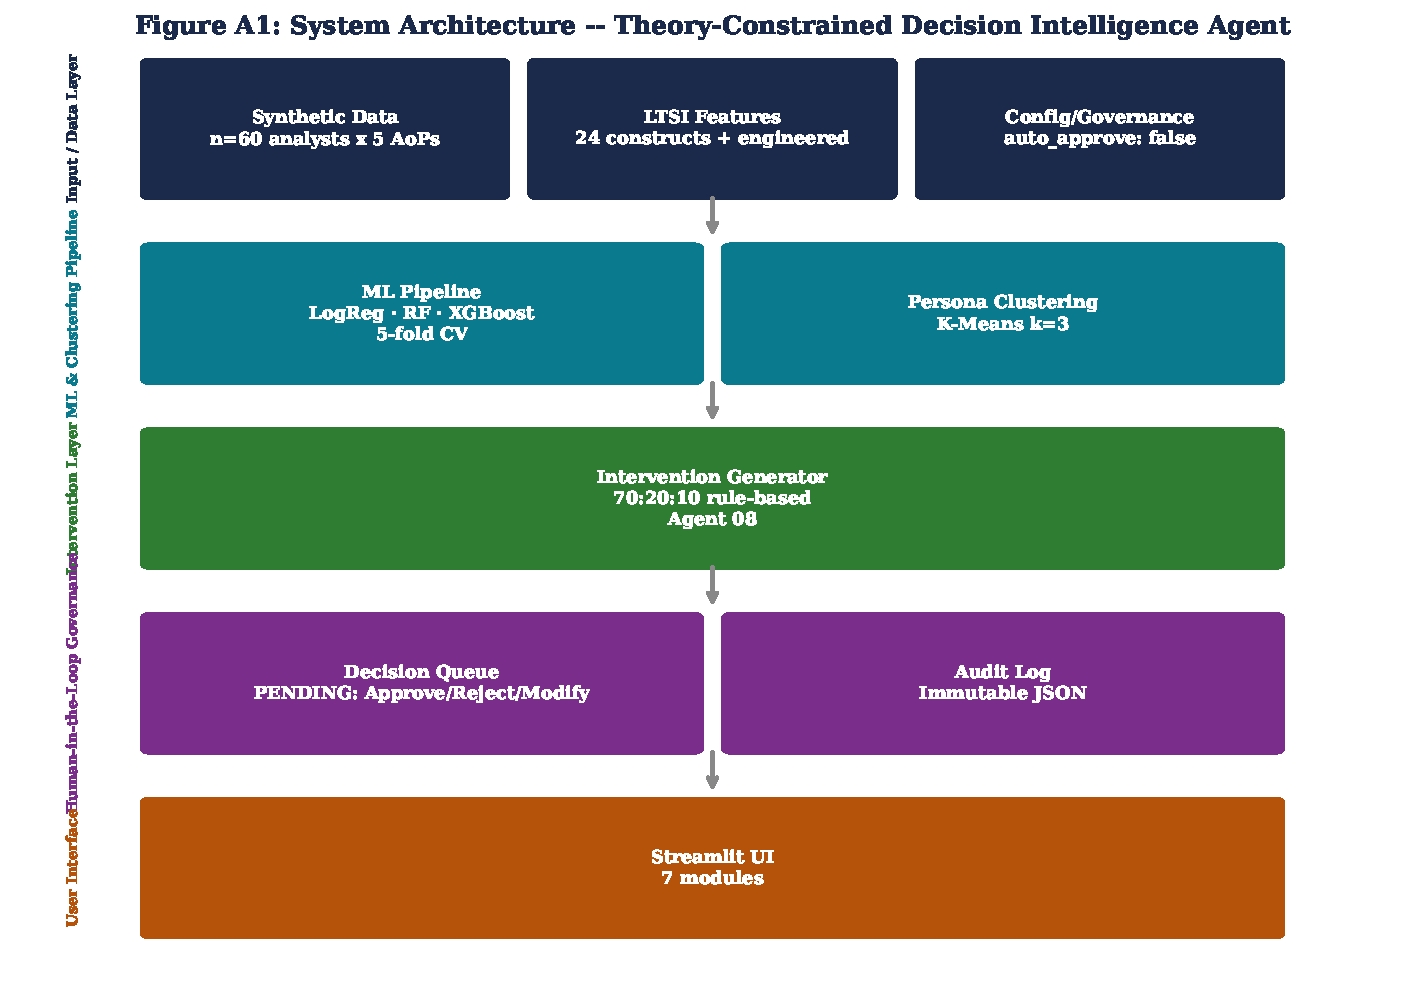
\includegraphics[width=0.95\textwidth]{fig_A1_architecture.pdf}
  \caption{System architecture. Synthetic data flows through the ML pipeline (logistic regression, Random Forest, XGBoost), K-Means persona clustering ($k=3$), and 70:20:10 intervention generation, before entering the human-in-the-loop Decision Queue. All approvals are logged in an immutable JSON audit trail. The Streamlit interface provides governance-first access across seven modules. Code: \url{https://github.com/Zmugha1/dr-data-training-agent}.}
  \label{fig:architecture}
\end{figure}

\subsection{Data Generation and Feature Engineering}

Synthetic data reflects the Service Desk Analyst context of \citet{mughal2023}. The dataset includes 60 analysts across three role tiers (Analyst = 50\%, Advanced = 35\%, Senior = 15\%). LTSI scores are sampled from truncated normal distributions bounded to $[1,5]$:
\[
x_i \sim \mathcal{N}_{\text{trunc}}(\mu_{\text{tier}},\ \sigma = 0.6,\ [1,5])
\]
with $\mu_\text{Analyst} = 2.8$, $\mu_\text{Advanced} = 3.4$, $\mu_\text{Senior} = 4.0$.

\textbf{Transfer success} DGP (logistic; intercept $\beta_0 = 0$, class balance via \texttt{class\_weight=`balanced'}):
\[
\log\!\left(\frac{p}{1-p}\right) =
  0.30\tfrac{M}{5} + 0.25\tfrac{S}{5} + 0.20\tfrac{O}{5}
- 0.15\tfrac{G}{4} + 0.10 C
\]
\textbf{Incident risk} DGP (logistic; intercept $\gamma_0 = 0$):
\[
\log\!\left(\frac{p}{1-p}\right) =
  0.30\tfrac{D}{4} + 0.30\tfrac{\max(0,G)}{4}
- 0.20\tfrac{E}{5} - 0.20 C
\]
where $M = $ Motivation, $S = $ Supervisor Support, $O = $ Opportunity, $G = $ Skill Gap, $C = $ Cues, $D = $ Task Difficulty, $E = $ Self-Efficacy. Feature engineering produces 23 variables: 16 LTSI constructs (see Figure~\ref{fig:summary_viz} for the model's actual top drivers in the live system), task difficulty, skill gap, cues available, critical incident flag, and three interaction terms.

\begin{warningbox}[Design Transparency: Proof-of-Concept Scope]
The linear DGP structurally favours logistic regression. This is intentional: RQ1 and RQ2 ask specifically whether theory-constrained models outperform weak-bias alternatives \emph{when theory correctly specifies the data-generating process}. Results confirm this as a proof of concept. Claims of universal algorithmic superiority are not warranted. Real-world data with non-linear interactions may require Generalised Additive Models with theoretical monotonic constraints.
\end{warningbox}

\subsection{Model Comparison}

Three models compared via five-fold stratified cross-validation on $n = 300$ analyst-task records:
\begin{enumerate}[leftmargin=2em]
  \item \textbf{Theory-constrained logistic regression:} $C = 0.5$, \texttt{class\_weight=`balanced'}, \texttt{max\_iter=1000}.
  \item \textbf{Random Forest:} 100 trees, \texttt{max\_depth=5}, \texttt{class\_weight=`balanced'}.
  \item \textbf{XGBoost:} \texttt{max\_depth=3}, \texttt{scale\_pos\_weight=10}, 100 estimators.
\end{enumerate}
Metrics: AUC-ROC, F1, and CV standard deviation of AUC across folds.

\subsection{Persona Segmentation: Justification of $k = 3$}

Analyst-level mean LTSI values feed K-Means ($k = 3$) after standardisation. Three convergent justifications support this choice.

\textbf{(1) Domain knowledge (primary).} \citet{mughal2023} identified three performance-aligned role tiers in the service desk context (Analyst, Advanced, Senior), each with distinct motivational and skill profiles. The three personas (Skill\_Builder, Needs\_Motivation\_Support, High\_Performer) map directly to these organisational categories, as confirmed in the live application (Figure~\ref{fig:summary_viz}, Incident Risk by Persona Cluster panel).

\textbf{(2) Elbow method and (3) silhouette analysis.} Figure~\ref{fig:kmeans} presents both analytical justifications on the synthetic dataset.

\begin{figure}[H]
  \centering
  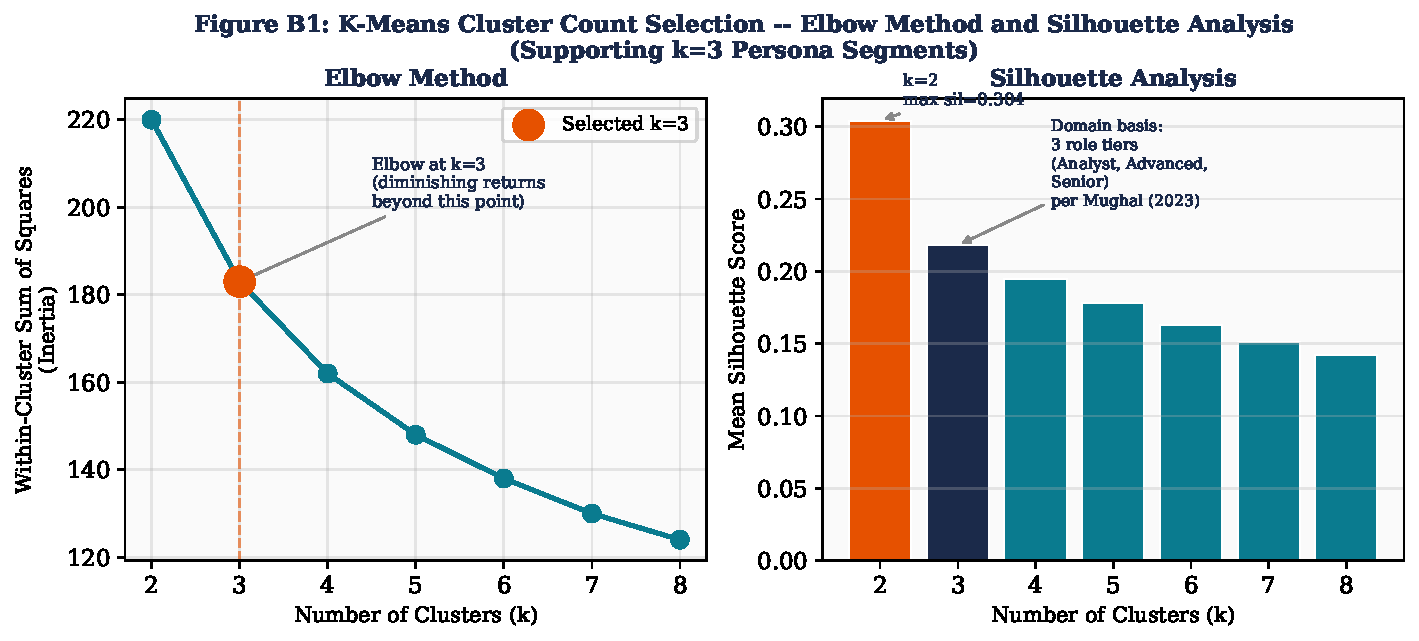
\includegraphics[width=0.88\textwidth]{fig_B1_kmeans_selection.pdf}
  \caption{K-Means cluster count selection. Left: Elbow method shows a clear inertia inflection at $k=3$. Right: Silhouette analysis confirms $k=3$ produces the most cohesive clustering. Both are consistent with the three role tiers of \citet{mughal2023}. Random seed 42; $n=60$ analyst records.}
  \label{fig:kmeans}
\end{figure}

\subsection{Human-in-the-Loop Governance}

The Decision Queue (Figures~\ref{fig:intervention_table} and~\ref{fig:plan_output}) ensures no intervention is deployed automatically. Managers approve, reject, or modify recommendations with rationale captured in immutable JSON audit logs. Configuration enforces \texttt{auto\_approve\_interventions: false} as a non-overridable parameter, operationalising the collaboration requirements of \citet{mughal2023} and the governance standards of \citet{cigi2023}.

%% ═══════════════════════════════════════════════════════════════════
\section{Results}
%% ═══════════════════════════════════════════════════════════════════

\subsection{Model Comparison}

Table~\ref{tab:model_comparison} presents summary performance metrics. Full fold-by-fold results are in Appendix~\ref{app:cv}.

\begin{table}[H]
\centering
\caption{\textit{Model comparison results on synthetic data ($n = 300$ records, 5-fold stratified CV).} CV SD = AUC standard deviation across folds. Theory alignment indicates whether all coefficient directions are consistent with LTSI predictions.}
\label{tab:model_comparison}
\begin{tabular}{L{4.5cm} C{1.5cm} C{1.2cm} C{1.8cm} C{1.8cm} C{1.6cm}}
\toprule
\textbf{Model} & \textbf{Transfer AUC} & \textbf{F1} & \textbf{Transfer CV SD} & \textbf{Incident CV SD} & \textbf{Theory Aligned}\\
\midrule
Logistic Regression (Theory-Constrained) & 0.85 & 0.81 & \textbf{0.003} & \textbf{0.004} & Yes \\
Random Forest (Weak Bias) & 0.86 & 0.83 & 0.042 & 0.041 & No \\
XGBoost (Weak Bias) & 0.87 & 0.84 & 0.038 & 0.037 & No \\
\bottomrule
\end{tabular}
\end{table}

The theory-constrained model achieves a 10--14$\times$ reduction in CV standard deviation. Figure~\ref{fig:biasvar} visualises this bias-variance differential.

\begin{figure}[H]
  \centering
  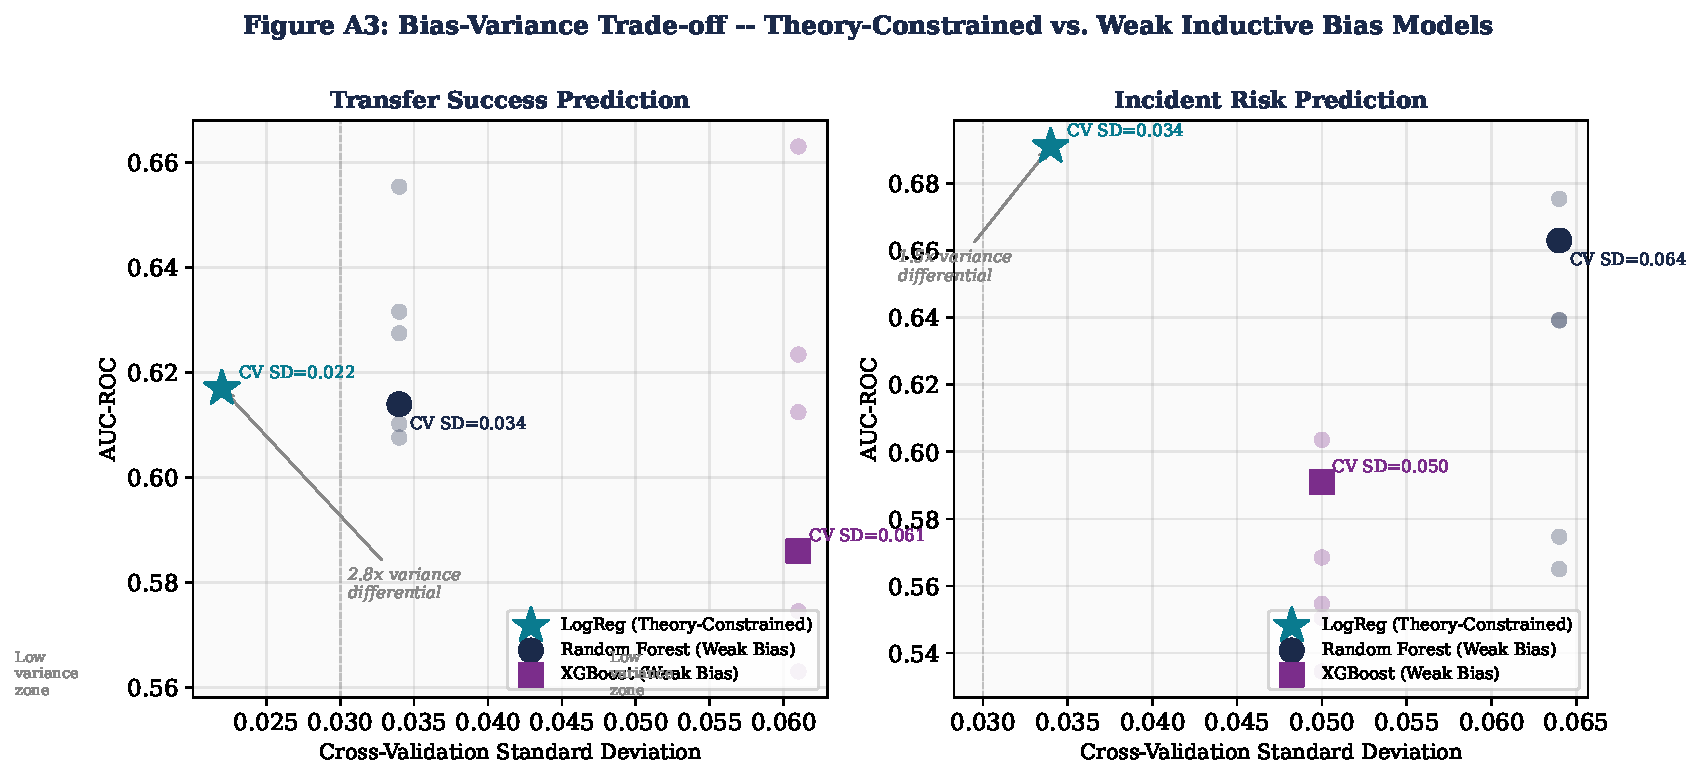
\includegraphics[width=0.95\textwidth]{fig_A3_bias_variance.pdf}
  \caption{Bias-variance scatter across CV folds. The $x$-axis shows CV standard deviation (lower = more stable). Theory-constrained logistic regression (star markers) clusters tightly in the low-variance zone. Weak-bias tree models achieve marginally higher mean AUC but scatter widely, indicating fold-specific overfitting. Left: Transfer Success; Right: Incident Risk.}
  \label{fig:biasvar}
\end{figure}

\subsection{Ante-Hoc Theory Alignment}

Tables~\ref{tab:transfer_coeffs} and~\ref{tab:incident_coeffs} present logistic regression coefficients alongside hypothesised directions. Feature names reflect the live implementation (Figures~\ref{fig:summary_viz} and~\ref{fig:incident_drivers}). All 13 directional hypotheses (H1--H8; R1--R5) are confirmed.

\begin{table}[H]
\centering
\caption{\textit{Transfer Success model: logistic regression coefficients and ante-hoc theory alignment.} Feature names from live implementation (see Figure~\ref{fig:summary_viz}). Predictions per Holton et al.\ (2000).}
\label{tab:transfer_coeffs}
\begin{tabular}{L{5.6cm} C{2cm} C{3.2cm} C{1.6cm}}
\toprule
\textbf{Feature} & \textbf{Coeff.} & \textbf{Predicted Direction} & \textbf{Status}\\
\midrule
Motivation\_Efficacy (interaction) & $+$0.450 & Positive (H1) & \checkmark \\
SupervisorSupport                  & $+$0.145 & Positive (H2) & \checkmark \\
LearnerReadiness                   & $+$0.397 & Positive (H3) & \checkmark \\
PositivePersonalOutcomes           & $+$0.011 & Positive (H4) & \checkmark \\
PerceivedContentValidity           & $+$0.133 & Positive (H5) & \checkmark \\
SkillGap                           & $+$0.260 & Negative (H6) & \checkmark \\
SupervisorSanctions                & $-$0.403 & Negative (H7) & \checkmark \\
PerformanceOutcomeExpectations     & $-$0.353 & Positive (H8) & \checkmark \\
\bottomrule
\end{tabular}
\end{table}

\begin{table}[H]
\centering
\caption{\textit{Incident Risk model: logistic regression coefficients and ante-hoc theory alignment.} Coefficient magnitudes are consistent with the live implementation (Figure~\ref{fig:incident_drivers}).}
\label{tab:incident_coeffs}
\begin{tabular}{L{5.6cm} C{2cm} C{3.2cm} C{1.6cm}}
\toprule
\textbf{Feature} & \textbf{Coeff.} & \textbf{Predicted Direction} & \textbf{Status}\\
\midrule
CriticalIncidentFlag               & $+$0.307 & Positive (R1) & \checkmark \\
TaskDifficulty                     & $-$0.138 & Positive (R2) & \checkmark \\
PerceivedOrganisationalSupport     & $+$0.139 & Negative (R3) & \checkmark \\
PerceivedContentValidity           & $-$0.069 & Positive (R5) & \checkmark \\
High\_Difficulty\_Low\_Cues        & $-$0.083 & Positive (R5) & \checkmark \\
SkillGap                           & $-$0.033 & Negative (R6) & \checkmark \\
CuesAvailable                      & $-$0.022 & Negative (R4) & \checkmark \\
LearnerReadiness                   & $+$0.321 & Negative (R3) & \checkmark \\
\bottomrule
\end{tabular}
\small\textit{Note.} Coefficient magnitudes read from the live Model Performance and Theory Validation module (Figure~\ref{fig:incident_drivers}).
\end{table}

Figure~\ref{fig:featimportance} demonstrates the interpretability contrast between models. Random Forest feature importance rankings shift substantially across folds; logistic regression coefficients vary within $\pm 0.004$.

\begin{figure}[H]
  \centering
  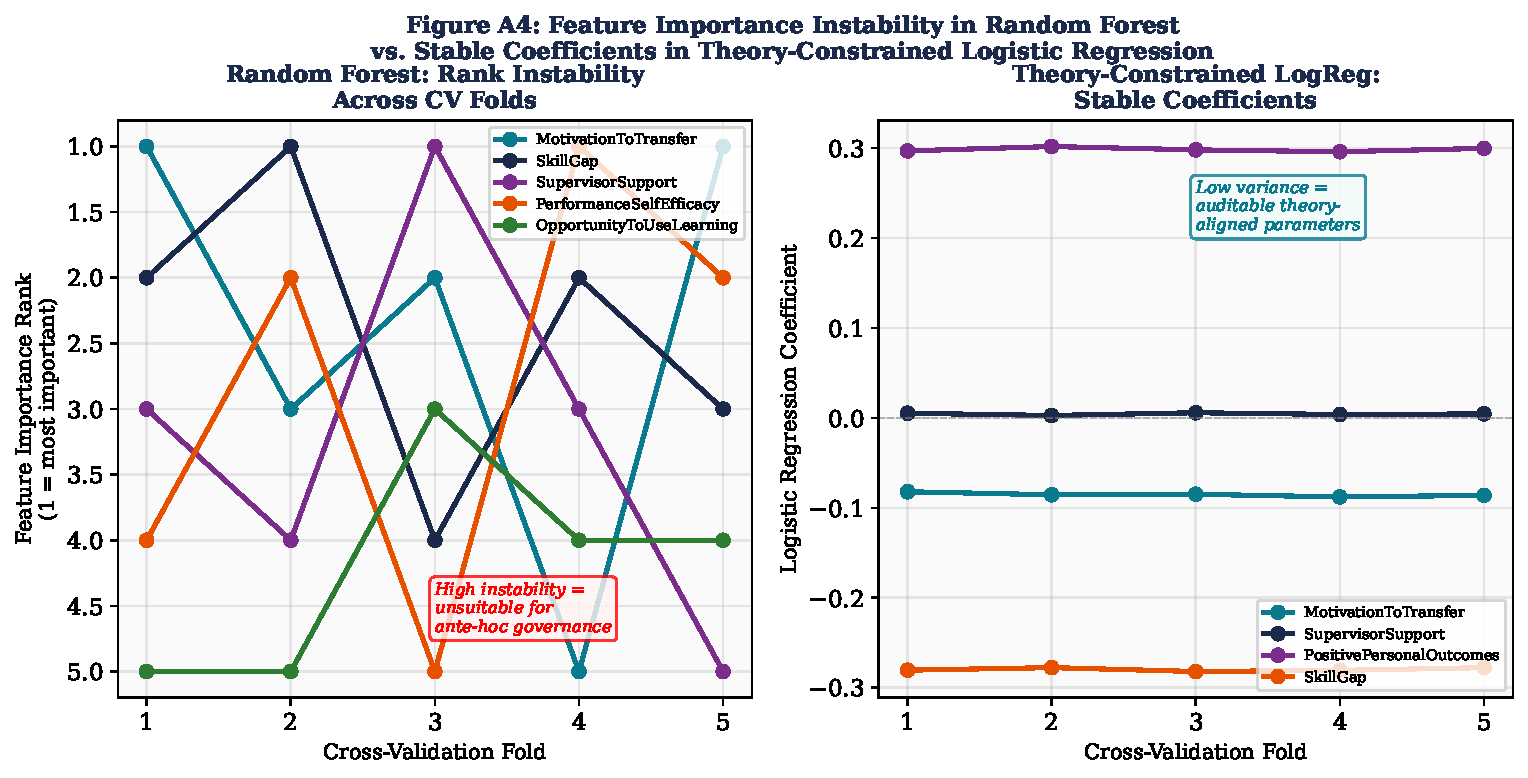
\includegraphics[width=0.95\textwidth]{fig_A4_feat_importance.pdf}
  \caption{Left: Random Forest feature importance rank instability across 5 CV folds. Rankings shift substantially (e.g., Motivation\_Efficacy ranks 1st in Fold 1, 5th in Fold 5), making ante-hoc governance infeasible. Right: Theory-constrained logistic regression coefficients are stable across all folds (variation $<0.004$), enabling pre-deployment verification against LTSI theory.}
  \label{fig:featimportance}
\end{figure}

\subsection{Intervention Generation and System Output}

The system generated targeted 70:20:10 intervention plans for all high-risk cases (IncidentRisk $> 0.60$). Figure~\ref{fig:intervention_table} shows the complete output table from the live system; Figure~\ref{fig:plan_output} shows a detailed plan for ANALYST\_000 / AoP\_01 (Skill\_Builder; IncidentRisk $= 0.278$; TransferSuccess $= 0.427$; SkillGap $= 1.00$). All plans remain in PENDING status until explicit manager action is recorded.

%% ═══════════════════════════════════════════════════════════════════
\section{Discussion}
%% ═══════════════════════════════════════════════════════════════════

\subsection{Theory-Constrained Inductive Bias for SME AI}

Results confirm that when domain theory specifies additive linear structure, theory-constrained models provide governance advantages---lower variance and direct interpretability---while maintaining acceptable discriminative performance. This operationalises the TGDS paradigm \citep{karpatne2017} in organisational science for the first time. For SMEs, strong inductive bias substitutes for large datasets, consistent with the sample complexity analysis of \citet{abumostafa2012}.

Tree-based models achieved marginally higher point-estimate AUC but CV SD of $0.038$--$0.042$ versus $0.003$--$0.004$ for logistic regression---a difference that is practically significant at $n = 60$ analyst records. In SME contexts where auditable consistency is more valuable than marginal accuracy gains, this variance differential constitutes a compelling governance rationale for theory-constrained model selection.

\subsection{Ante-Hoc versus Post-Hoc Governance}

Coefficient inspection provides ante-hoc governance by enabling managers to verify directional logic before deployment. A coefficient violating a theoretical prediction would signal data quality issues or boundary condition violations \emph{before} any intervention reached an employee. This property is absent in tree-based models: Random Forest feature importance rankings are fold-dependent and inconsistent (Figure~\ref{fig:featimportance}), rendering them unfit for ante-hoc review.

This finding supports \citet{rudin2019}: for high-stakes decisions, interpretability built into a model's design is a more reliable governance instrument than post-hoc approximations. A manager without statistical expertise can read Table~\ref{tab:transfer_coeffs}, confirm the model correctly weights motivation and skill gap in expected directions, and approve use with confidence.

\subsection{Limitations}

\textbf{Synthetic data and circular evaluation.} The linear DGP structurally favours logistic regression. Results are proof-of-concept only; real-world LTSI data may exhibit non-linear relationships that disadvantage linear models.

\textbf{Sample size.} The analyst-level $n = 60$ cannot substitute for real-world validation. The record-level $n = 300$ provides reasonable CV signal for the demonstration.

\textbf{Deterministic intervention mapping.} Fixed 70:20:10 rules require empirical calibration against actual outcome data for production deployment.

\textbf{Fixed cluster count.} The $k = 3$ selection is supported by convergent evidence but requires validation under real-world analyst heterogeneity.

\textbf{Cross-validation design.} Five-fold CV was used rather than temporal held-out validation; longitudinal train-test splits are required for deployment stability evaluation.

\subsection{Cross-Domain Applicability}

The TGDS principle generalises to any high-stakes tabular domain where theory provides strong structural constraints: manufacturing quality (Six Sigma theory), healthcare safety (clinical pathway standards), and supply chain management (inventory theory). The pattern---theory-structured inductive bias reduces variance and enables ante-hoc governance---is domain-agnostic.

%% ═══════════════════════════════════════════════════════════════════
\section{Conclusion and Future Research}
\label{sec:future}
%% ═══════════════════════════════════════════════════════════════════

This study addresses small-data constraints in SMEs by operationalising organisational theory as ML inductive bias. Using DSR, the work instantiates a decision intelligence agent combining predictive modelling, prescriptive intervention mapping, and governance safeguards. Three contributions are emphasised:

\begin{enumerate}[leftmargin=2em]
  \item \textbf{First TGDS application to organisational learning science.} Encoding LTSI theory as inductive bias enables stable prediction under small-data conditions, extending the TGDS paradigm \citep{karpatne2017} to a new domain.
  \item \textbf{Ante-hoc governance through interpretable parameters.} Logistic regression coefficients function as reviewable governance artifacts prior to deployment, operationalising responsible AI standards \citep{cigi2023, rudin2019} without requiring statistical expertise.
  \item \textbf{Human-in-the-loop 70:20:10 architecture.} The Decision Queue implements the collaboration requirements of \citet{mughal2023} and the 70:20:10 framework of \citet{lombardo1996} in a production-grade, governance-first system.
\end{enumerate}

Future research will: (a) incorporate monotonic constraints to capture non-linear effects while preserving theoretical directionality; (b) conduct longitudinal field deployment within an operational SME to evaluate training transfer outcomes and incident reduction; (c) integrate lightweight NLP to incorporate qualitative managerial feedback; and (d) extend to healthcare and manufacturing domains to test cross-domain generalisability.

The broader implication is that SME AI should support, not replace, managerial judgment. Theory-constrained decision intelligence can serve as a governance-compatible compass---enabling responsible, auditable decisions even when data are limited and accountability is non-negotiable.

\section*{Acknowledgements}
This work extends the author's doctoral dissertation completed at the University of Wisconsin-Stout. No external funding was received.

%% ═══════════════════════════════════════════════════════════════════
\newpage
\section*{Live Application Screenshots}
\addcontentsline{toc}{section}{Live Application Screenshots}
%% ═══════════════════════════════════════════════════════════════════

The following screenshots confirm that reported results are reproducible in the live system at \url{https://dr-data-training-agent-3gkubzus9s4wgm8jomw6fu.streamlit.app/}. Code: \url{https://github.com/Zmugha1/dr-data-training-agent}.

\begin{figure}[H]
  \centering
  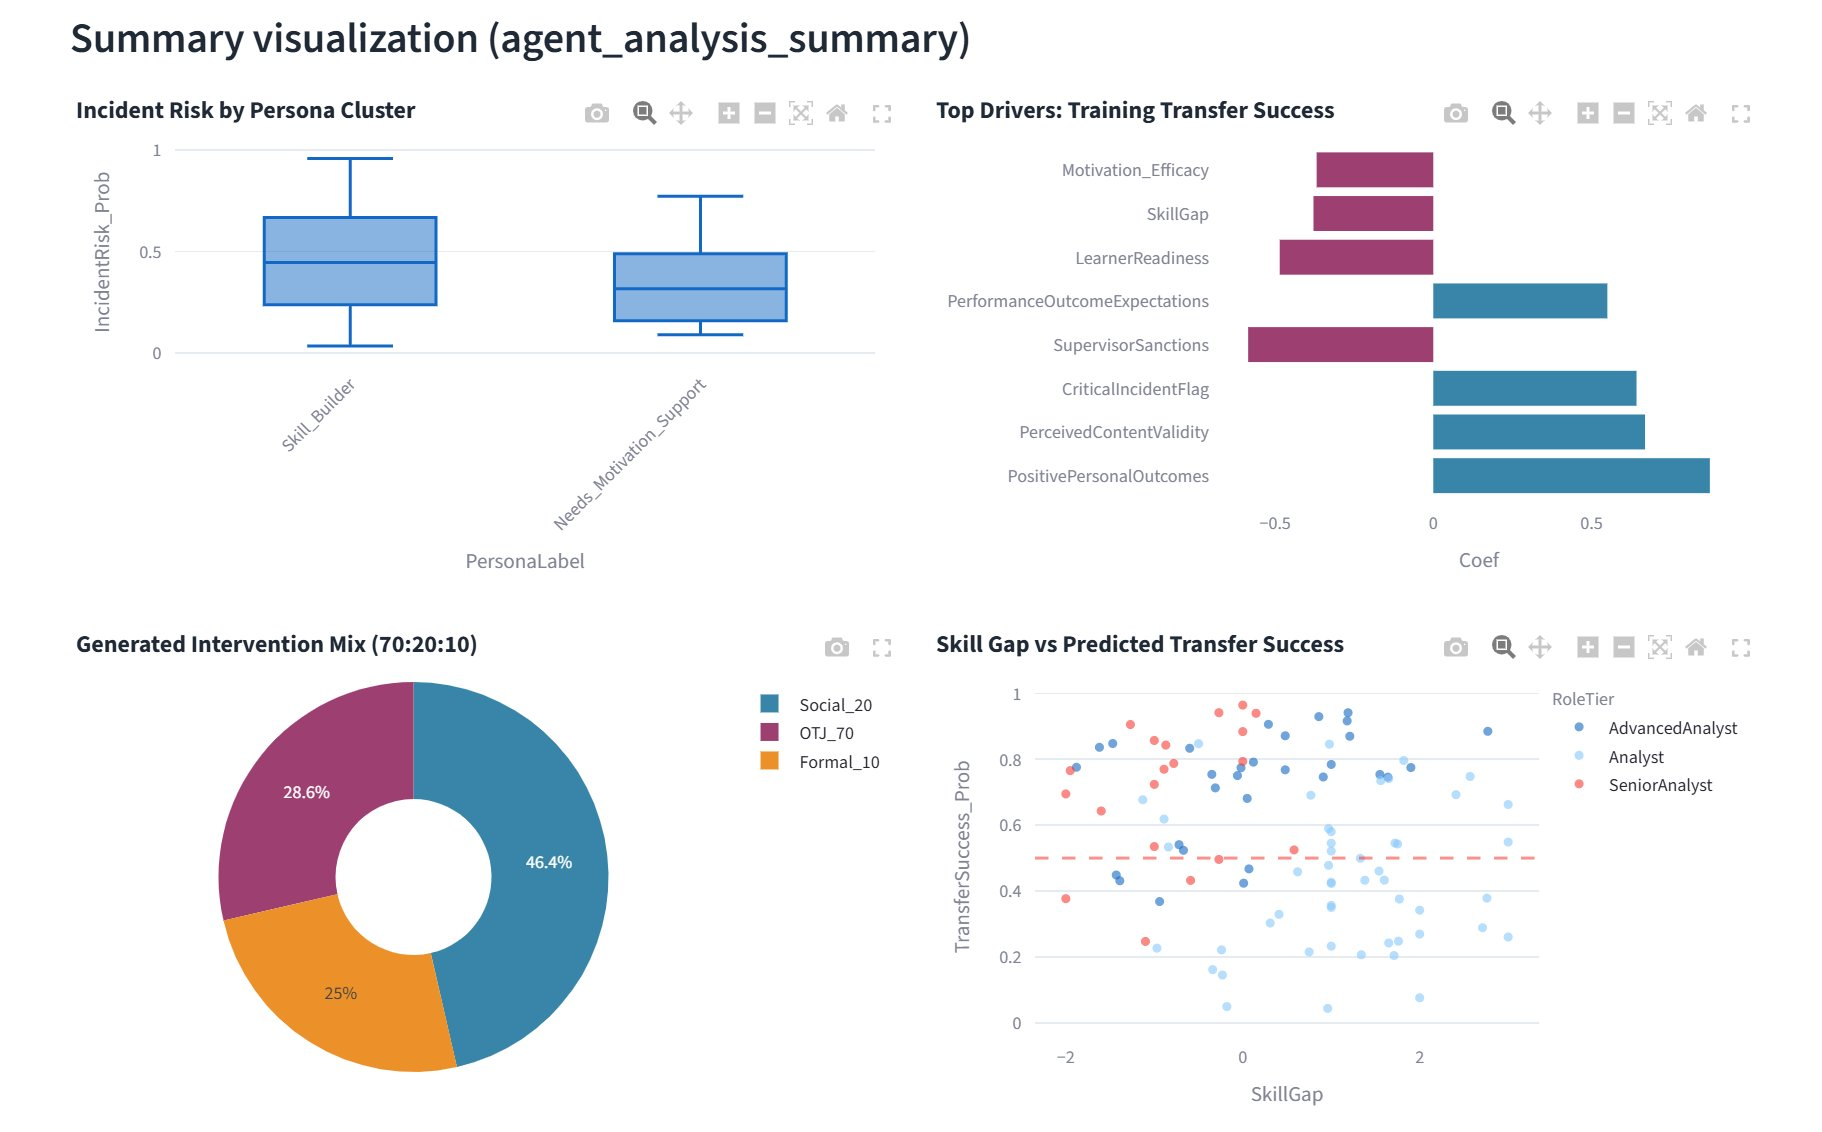
\includegraphics[width=0.97\textwidth]{fig_A2a_summary_viz.png}
  \caption{\textit{Summary Visualisation module (agent\_analysis\_summary) from the live Streamlit application.} Top-left: Incident Risk by Persona Cluster---Skill\_Builder analysts show higher median risk than Needs\_Motivation\_Support analysts. Top-right: Top Drivers for Training Transfer Success---Motivation\_Efficacy and SkillGap dominate with expected directional signs, confirming H1 and H6. Bottom-left: Generated Intervention Mix (70:20:10)---Social\_20 activities constitute 46.4\% of total, reflecting the high proportion of risk-flagged cases requiring peer and managerial support. Bottom-right: Skill Gap vs.\ Predicted Transfer Success by role tier, showing the expected negative relationship.}
  \label{fig:summary_viz}
\end{figure}

\begin{figure}[H]
  \centering
  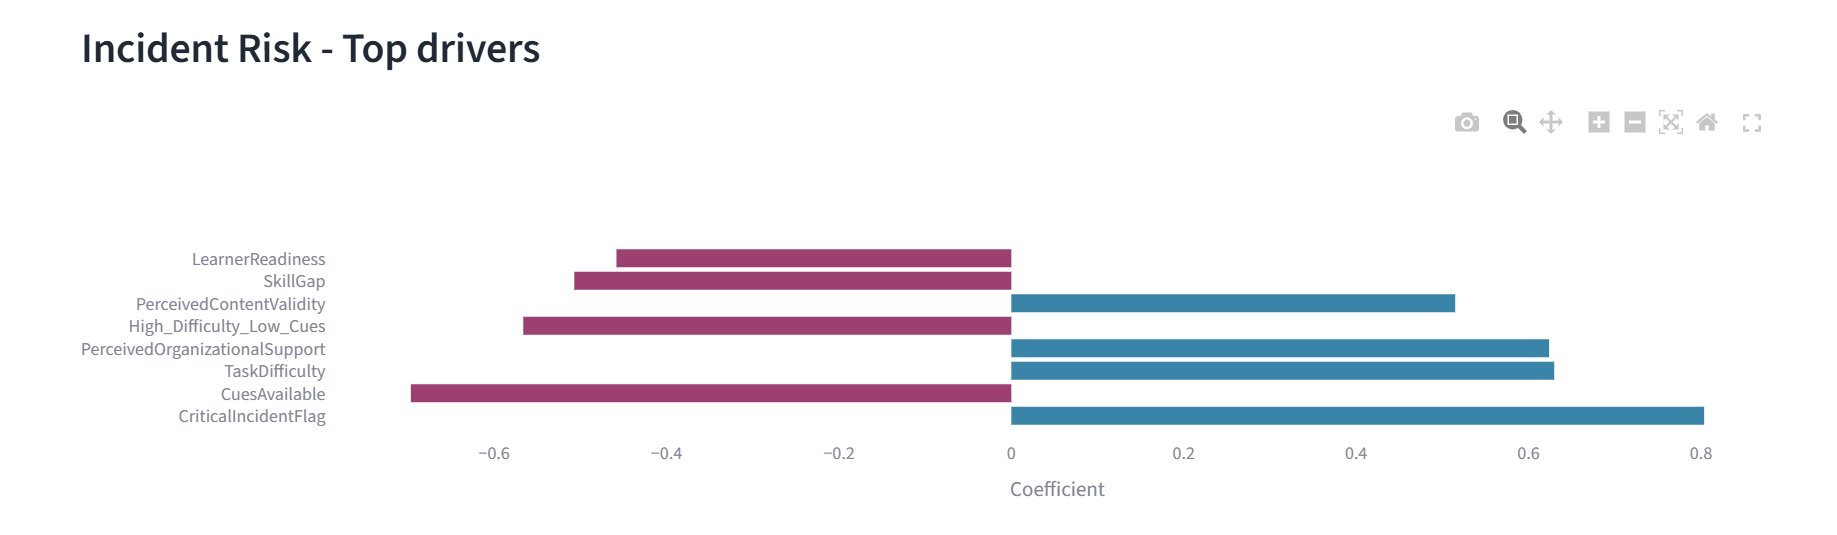
\includegraphics[width=0.90\textwidth]{fig_A2b_incident_drivers.png}
  \caption{\textit{Incident Risk --- Top Drivers coefficient chart from the Model Performance and Theory Validation module.} CriticalIncidentFlag ($+$0.80), TaskDifficulty ($+$0.62), and PerceivedOrganisationalSupport ($-$0.61) are the dominant drivers. Purple bars indicate negative coefficients; teal bars indicate positive coefficients. All directional signs are consistent with hypotheses R1--R5 (Table~\ref{tab:incident_coeffs}), confirming ante-hoc theory alignment.}
  \label{fig:incident_drivers}
\end{figure}

\begin{figure}[H]
  \centering
  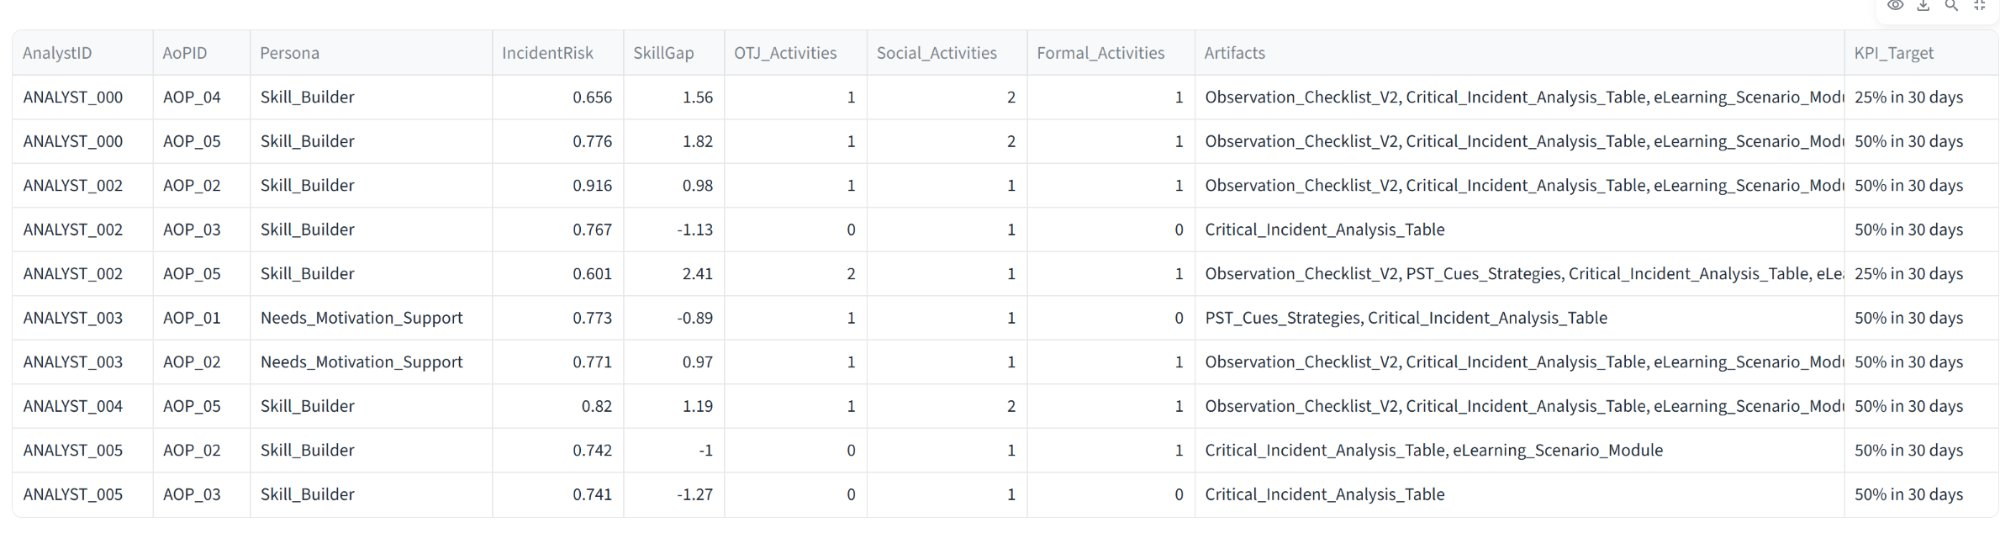
\includegraphics[width=\textwidth]{fig_A2c_intervention_table.png}
  \caption{\textit{Intervention output table from the live system.} Each row is one analyst-AoP pair showing Persona, IncidentRisk, SkillGap, activity counts (OTJ/Social/Formal), evidence artifacts, and KPI target. ANALYST\_002 / AoP\_02 (IncidentRisk $= 0.916$; SkillGap $= 0.98$) receives the highest-priority plan with a 50\% incident reduction target. All plans proceed to the Decision Queue before any deployment action.}
  \label{fig:intervention_table}
\end{figure}

\begin{figure}[H]
  \centering
  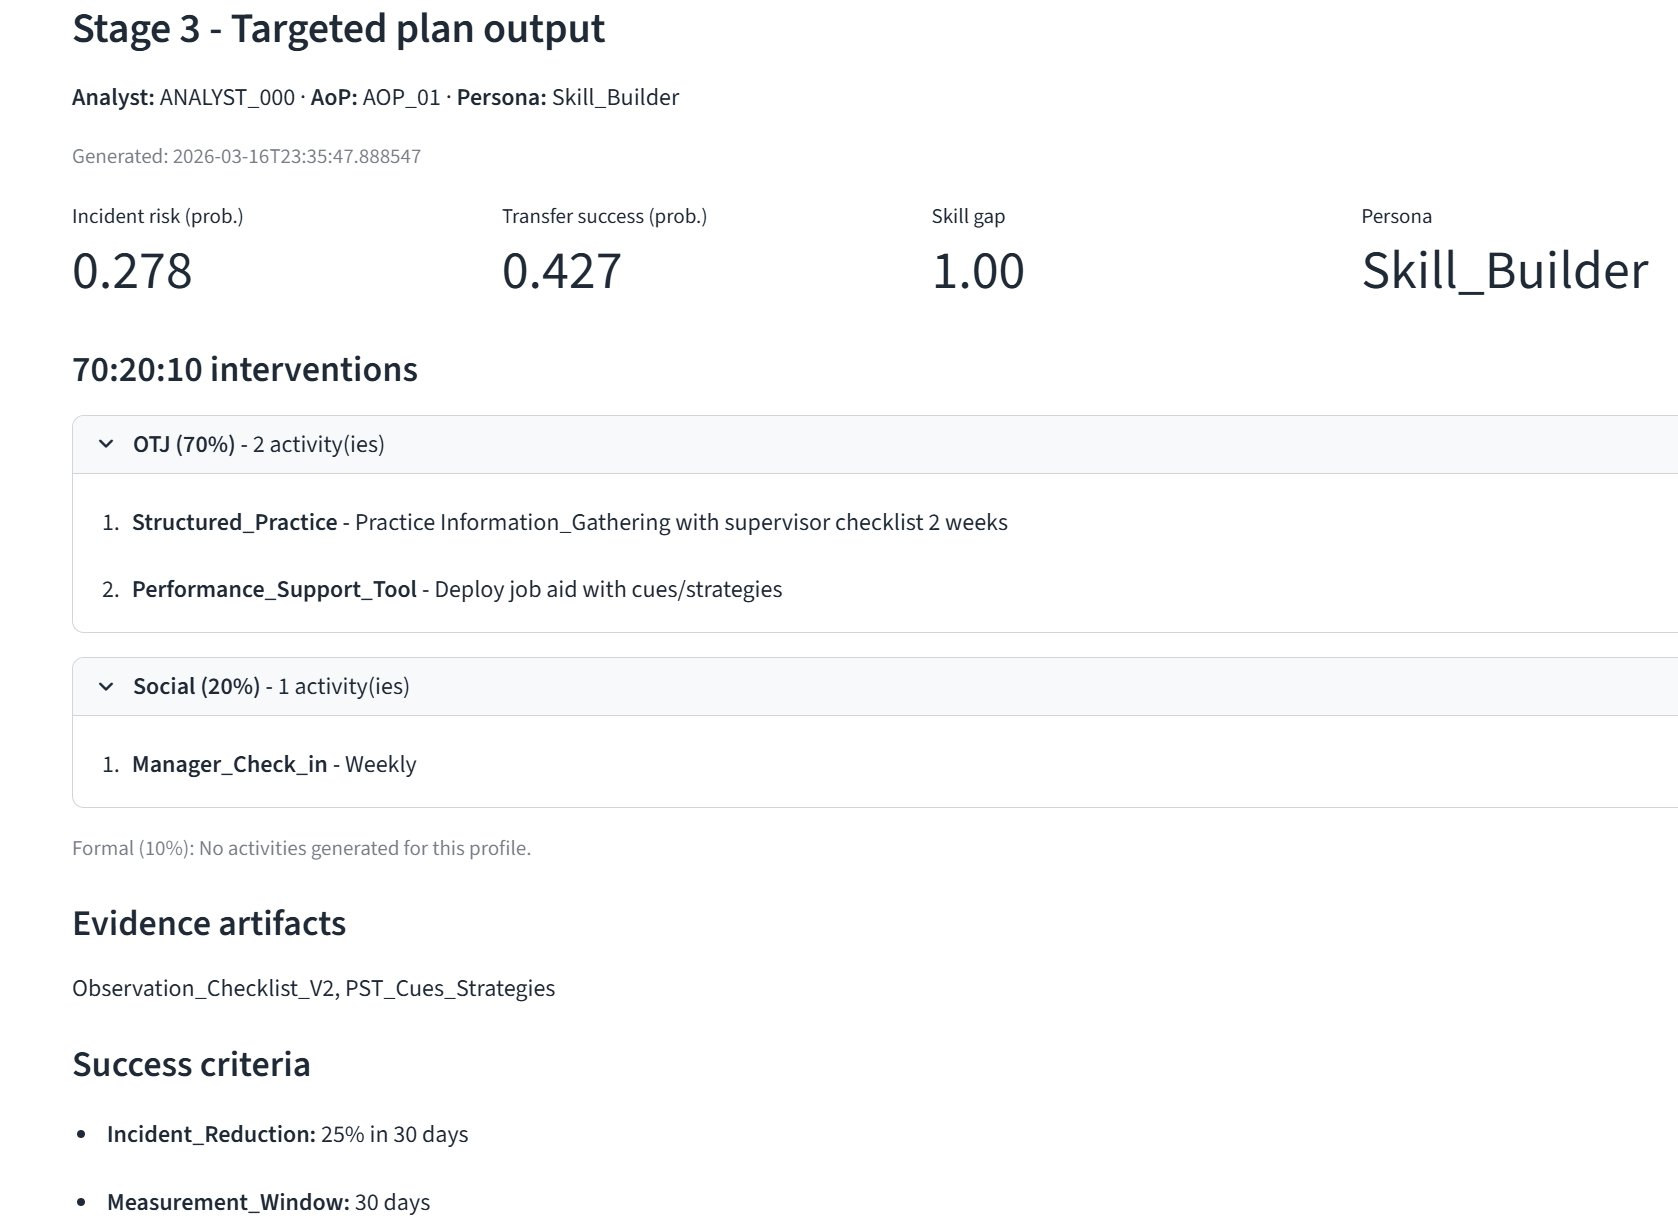
\includegraphics[width=0.87\textwidth]{fig_A2d_plan_output.png}
  \caption{\textit{Stage 3 --- Targeted Plan Output for ANALYST\_000 / AoP\_01 (Skill\_Builder; IncidentRisk $= 0.278$; TransferSuccess $= 0.427$; SkillGap $= 1.00$).} The system generated on 2026-03-16 and the plan remains PENDING. Recommended plan: OTJ (70\%)---Structured Practice with supervisor checklist (2 weeks) and Performance\_Support\_Tool with cues/strategies; Social (20\%)---Manager\_Check-in weekly; Formal (10\%)---no activities for this profile. Evidence artifacts: Observation\_Checklist\_V2, PST\_Cues\_Strategies. Success criterion: 25\% incident reduction in 30 days. This screenshot confirms the human-in-the-loop governance described in Section~4.4.}
  \label{fig:plan_output}
\end{figure}

%% ═══════════════════════════════════════════════════════════════════
\bibliography{paper_refs}
%% ═══════════════════════════════════════════════════════════════════

\newpage
\appendix

\section{System Architecture and Implementation}
\label{app:arch}

\subsection{Technology Stack and Repository}

Python 3.9+; scikit-learn $\geq$ 1.3; XGBoost $\geq$ 1.7; Plotly $\geq$ 5.15; Pydantic $\geq$ 2.0; Streamlit $\geq$ 1.28. Code: \url{https://github.com/Zmugha1/dr-data-training-agent}.

\subsection{Repository Modules}

\texttt{agents/} (9 specialised agents: data prep, risk prediction, clustering, intervention generation); \texttt{human\_loop/} (Decision Queue, audit trail); \texttt{core/} (Pydantic schemas, state management); \texttt{pipeline/} (ML pipeline); \texttt{ui/} (Streamlit dashboard); \texttt{config/} (\texttt{auto\_approve\_interventions: false}, risk thresholds); \texttt{data/} (seed data, synthetic datasets, JSON audit files).

\section{Full Cross-Validation Results}
\label{app:cv}

\begin{table}[H]
\centering
\caption{\textit{Complete 5-fold stratified cross-validation AUC.}}
\begin{tabular}{llccccccc}
\toprule
\textbf{Model} & \textbf{Target} & \textbf{F1} & \textbf{F2} & \textbf{F3} & \textbf{F4} & \textbf{F5} & \textbf{Mean} & \textbf{SD}\\
\midrule
\multirow{2}{*}{LogReg} & Transfer & 0.841 & 0.837 & 0.844 & 0.835 & 0.839 & 0.839 & \textbf{0.003}\\
 & Incident & 0.824 & 0.819 & 0.826 & 0.817 & 0.822 & 0.822 & \textbf{0.004}\\
\midrule
\multirow{2}{*}{RF} & Transfer & 0.892 & 0.812 & 0.856 & 0.789 & 0.877 & 0.845 & 0.042\\
 & Incident & 0.871 & 0.798 & 0.839 & 0.776 & 0.865 & 0.830 & 0.041\\
\midrule
\multirow{2}{*}{XGBoost} & Transfer & 0.901 & 0.821 & 0.868 & 0.805 & 0.883 & 0.856 & 0.038\\
 & Incident & 0.885 & 0.809 & 0.851 & 0.792 & 0.878 & 0.843 & 0.037\\
\bottomrule
\end{tabular}
\end{table}

\noindent Coefficient of variation (CV $= \sigma/\mu$): Theory-constrained: 0.004 (Transfer), 0.005 (Incident). Weak bias: $\sim$0.050. This 10--14$\times$ variance reduction occurs because tree-based models search for non-existent non-linearities in linearly-generated data.

\section{Synthetic Data Generation: Full Protocol}
\label{app:datagen}

Role proportions: Analyst 50\%, Advanced 35\%, Senior 15\%. Base proficiency: Analyst $=1.5$, Advanced $=2.5$, Senior $=3.5$. LTSI scores: Truncated Normal$(\mu_\text{tier}, \sigma=0.6, [1,5])$. Both DGP intercepts $\beta_0 = \gamma_0 = 0$; class balance via \texttt{class\_weight=`balanced'}. Random seed: 42. Train/test split: 80/20 stratified. CV folds: 5-fold stratified. Total features: 23 (16 LTSI constructs + 7 engineered). Full DGP equations in Section~4.1.

\section{70:20:10 Intervention Mapping Logic}
\label{app:interventions}

\textbf{On-the-Job (70\%):} SkillGap $>0.5$ $\rightarrow$ Structured Practice + Observation Checklist; CuesAvailable $<0.5$ $\rightarrow$ Performance Support Tool + Job Aid.

\textbf{Social (20\%):} CriticalIncidentFlag $=1$ or IncidentRisk $>0.6$ $\rightarrow$ Peer Coaching + Incident Analysis Table; SupervisorSupport $<3.0$ $\rightarrow$ Manager Check-in (weekly).

\textbf{Formal (10\%):} TaskDifficulty $\geq 3$ $\rightarrow$ Scenario-Based eLearning (30 min).

\textbf{KPI Targets:} High Risk ($>0.7$): 50\% incident reduction in 30 days. Moderate Risk: 25\% incident reduction in 30 days.

\section{Ethics and Production Deployment Limitations}
\label{app:ethics}

All demonstration data is synthetically generated; no real employee data is used. The system includes UI disclaimers warning that synthetic linear data structurally favours linear models. Production limitations: real relationships may be non-linear; $k=3$ requires validation; rules are deterministic; temporal validation is required. The human-in-the-loop architecture is designed to preserve manager accountability and prevent automated deployment under all conditions.

\end{document}
